% Integrals: the region D between y = x^2 (below) and y = x (above).
\documentclass[border=4pt]{standalone}
\usepackage{tikz}
\begin{document}
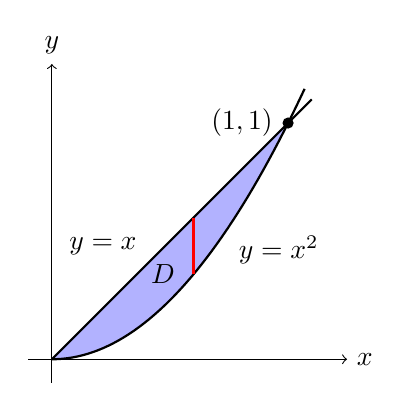
\begin{tikzpicture}[scale=3]
  \fill[blue!30] (0,0) -- plot[domain=0:1, samples=50] (\x,{\x*\x}) -- cycle;
  \draw[->] (-0.1,0) -- (1.25,0) node[right] {$x$};
  \draw[->] (0,-0.1) -- (0,1.25) node[above] {$y$};
  \draw[thick] (0,0) -- (1.1,1.1);
  \draw[thick, domain=0:1.07, samples=50] plot (\x,{\x*\x});
  \node[above left]  at (0.4,0.4)   {$y=x$};
  \node[below right] at (0.75,0.5625) {$y=x^2$};
  % A vertical strip: y runs from x^2 up to x.
  \draw[thick, red] (0.6,0.36) -- (0.6,0.6);
  \node at (0.47,0.36) {$D$};
  \filldraw (1,1) circle (.6pt) node[left=2pt] {$(1,1)$};
\end{tikzpicture}
\end{document}
